

\input{../Latex_Templates/Preamble_Report}

%%%%% TITLE PAGE

%\subject{, VT23}
\title{ Some title \\[1ex]
	  \large Master Thesis}
%\subtitle{}
\author{Theo Koppenhöfer}
\date{Lund \\[1ex] \today}

\addbibresource{bibliography.bib}

\usepackage{svg}
\graphicspath{{../Plots/}}
\graphicspath{{../Figures/}}

\pgfplotsset{
	compat=newest,
    every axis/.append style={
        axis y line=left,
        axis x line=bottom,
        scale only axis,
%    	max space between ticks=25pt,
        width=0.7\textwidth,
        scaled ticks=true,
        axis line style={thick,-,>=latex, shorten >=-.4cm},
    		x tick label style={
		    /pgf/number format/precision=3
		}
    },
    every axis plot/.append style={thick},
    tick style={black, thick}
}

\newcommand{\bx}{\bar{x}}

%%%%% The content starts here %%%%%%%%%%%%%


\begin{document}

\maketitle

\tableofcontents

\newpage

\listoftodos

\todoin[]{
  General TODOs
  \begin{itemize}
    \item Disproof using hairy ball theorem.
    \item Write other example
    \item Look what happens if you add the examples
    \item Check that the signs of the examples are correct
    \item Make the plots of the examples look nice.
    \item Change $n$ to $d$, consistent notation.
    \item Check for typos.
    \item Does Girault-Raviart theorem with Helmholtz decomp. help?
    \item bring in results from \cite{Shelton1980} and \cite{Morse1970}
  \end{itemize}
  Some questions
  \begin{itemize}
    \item Should I state Hopf's Lemma?
  \end{itemize}
}

\newpage

\section{Introduction}

\ruggedtodo[inline]{Some amazing introduction}

Unless otherwise stated we denote by $\Omega\subseteq\R^d$ an open bounded subset of $\R^d$ with boundary $\Sigma=\partial\Omega$.
We denote with
\begin{align*}
  f\colon\overline{\Omega}\to\R
\end{align*}
a scalar function of class $C^2$. We also denote by
\begin{align*}
  u\colon\overline{\Omega}\to\R^d
\end{align*}
a vector field of class $C^1$. Often but not always $u$ can be thought of as 
a \emph{harmonic vector field}, that is $u$ fulfils
\begin{align*}
  \diver u=0 \qquad \text{ and }\qquad \curl u=0\,.
\end{align*}
Also often but not always we assume that locally $u=\nabla f$, implying that $f$ is harmonic.
One question we seek to answer during this thesis is the following.
\begin{question}[Flowthrough with stagnation point]\label{qu:flowthroughStagnationPoint}
  Does there exist a tube $\Omega\subseteq\R^3$ with flow $u$ through the tube such that
  \begin{enumerate}
    \item $u$ is a harmonic vector field
    \item $u$ has an interiour stagnation point
    \item $u$ enters the tube on the one end and exits the tube on the other?
  \end{enumerate}
\end{question}
To make the formulation more precise we begin with some general definitions regarding stagnation points and the boundary conditions.

\subsection{General definitions}

In the following we define the emergent and the entrant boundary as in \cite[p.282]{Morse1970}
\begin{definition}[Emergent and entrant boundary]
  We call a vector $v\in T_x\R^d$ \emph{entrant} at a boundary point $x\in\Sigma$ iff $v$ is not tangent to $\Sigma$
  and directed into the interiour of $\Omega$. Analogously if $v$ is not tangent and
  directed to the exteriour we call $v$ \emph{emergent}.
  We define the \emph{entrant boundary} $\Sigma^-$ to be the set of boundary points at which $u$ is entrant.
  Analogously define the \emph{emergent boundary} $\Sigma^+$ to be the set of boundary points at which
  $u$ is emergent.
  Further define $\Sigma^0$ to contain all other boundary points such that we have a decomposition
  of the boundary
  \begin{align*}
    \Sigma=\Sigma^-\sqcup\Sigma^0\sqcup\Sigma^+\,.
  \end{align*}
\end{definition}

The following are slight generalisation of the definitions given in \cite[p.138f]{Shelton1980}, \cite[§5]{Morse1969} and \cite[p.282f]{Morse1970}
to include harmonic vector fields.
We call the zeroes of $u$ \emph{critical points}. A critical point $x\in\Omega$ is called
\emph{non-degenerate} if the derivative $Du(x)$ is invertible. We say that $x$ has \emph{index} $k$
if $Du(x)$ has exactly $k$ negative eigenvalues. $u$ is called \emph{non-degenerate} if all its critical points
are non-degenerate.

We now define the \emph{interiour type numbers} $M_k$
to be the number of critical points of $u$ of index $k$.
The total number of critical points is thus given by
\begin{align*}
  M=\sum_kM_k\,.
\end{align*}
We call $\Omega$ a \emph{regular domain} if $\Sigma$ is a manifold of class $C^2$.
In the following definition we require $\Omega$ to be regular.
\begin{definition}[Boundary type numbers]
  For a boundary point $x$ let $$\pi_x\colon \R^d\cong T_x\R^d\to T_x\Sigma$$ denote the projection of a
  vector at $x$ onto the tangent space of $\Sigma$ at $x$.
  Let $$u_{\Sigma^-}=\pi\circ u\vert_{\Sigma^-}\in C^1\brk*{T\Sigma^-}$$ be the restriction and projection of $u$ onto the tangent bundle of $\Sigma^-$.
  \ruggedtodo[]{This construction surely has a name in diffGeo.}
  We define the \emph{boundary type numbers} $\mu_k$ to be
  the number of critical points of $u_{\Sigma^-}$ on the entrant boundary
  $\Sigma^-$ of index $k$.
  We further write $\nu_k$ for the $k$-th boundary type number of $-u$.
\end{definition}

We now call $u$ \emph{regular} iff $u$ and $u_\Sigma$ are non-degenerate and all critical points lie in $\Omega$.

The previous definitions translate naturally to $f$.
We call $f$ regular, non-degenerate, et cetera iff $u=\nabla f$ is regular, non-degenerate, et cetera.


\subsection{On assuming non-degeneracy}


\section{Some general remarks}

\todoin[]{
\begin{itemize}
  \item only finitely many critical points possible
\end{itemize}
}

\subsection{Betti numbers}

For a formal definition of Betti numbers we refer to ??.
We do however give some examples of Betti numbers for some domains.
\ruggedtodo[inline]{complete this section}

\subsection{The Morse inequalities}

We state the Morse inequalities.\ruggedtodo[]{More citations.}
\begin{theorem}[Morse inequalities]
Let $\Omega$ and $f$ be regular. Then we have the inequalities
\begin{align*}
  0&\leq M_0+\mu_0-R_0\\
  0&\leq M_1+\mu_1-R_1-\brk*{M_0+\mu_0-R_0} \\
  &\;\;\vdots \\
  0&\leq M_{d-1}+\mu_{d-1}-R_{d-1}-\cdots +\brk*{-1}^{d-1}\brk*{M_0+\mu_0-R_0} \\
  0&=M_{d}-R_{d}-\brk*{M_{d-1}+\mu_{d-1}-R_{d-1}}+\cdots +\brk*{-1}^{d}\brk*{M_0+\mu_0-R_0}\,.
\end{align*}
\end{theorem}
\begin{proof}
  See \cite{Morse1969}.\ruggedtodo[]{Give a more precise reference.}
\end{proof}
If we now assume that $f$ is harmonic then the maximum principle implies that
$M_0=0=M_d$ and thus we obtain for the special case of dimensions $d=2$.
\begin{corollary}[Morse inequalities for $f$ harmonic, $d=2$]
  Let $d=2$, $\Omega$ and $f$ be regular and assume that $f$ is harmonic. Then we have
  \begin{align*}
    0&\leq \mu_0-R_0 \\
    0&=M+\mu_1-R_1-\mu_0+R_0\,.
  \end{align*}
\end{corollary}
In dimensions $d=3$ we obtain
\begin{corollary}[Morse inequalities for $f$ harmonic, $d=3$]
  Let $d=3$, $\Omega$ and $f$ be regular and assume that $f$ is harmonic. Then we have
  \begin{align*}
    0&\leq \mu_0-R_0 \\
    0&\leq M_1+\mu_1-R_1-\mu_0+R_0 \\
    0&= M_2+\mu_2-R_2-M_1-\mu_1+R_1-\mu_0+R_0\,.
  \end{align*}
\end{corollary}
\ruggedtodo[]{Introduce Morse inequalities for $-f$.}

\newpage

\section{Harmonic functions, $d=2$}

The following result is essentially a negative to question \ref{qu:flowthroughStagnationPoint} in $d=2$ dimensions.
\begin{proposition}\label{pr:n2:hf:nonExistence}
  Let $\Omega$ be homeomorphic to $B_1\subseteq\R^2$. Let further $f\colon\overline{\Omega}\to\R$ be regular harmonic  
  with critical point $x_1\in\Omega$. Then $\Sigma^-\subseteq\Sigma$ is not connected.
\end{proposition}
We shall give two different proofs of this result. One involving level-sets and the other involving invariant manifolds

\subsection{A proof involving level-sets}

\begin{proof}[Sketch of Proof.]
  Let $y_c=f(x_1)$ and $x_1,\dots,x_M$ be all the critical points such that $f(x_\cdot)=y_c$.
  We claim that the level set
  \begin{align*}
    C=\brk[c]*{f=y_c}\subseteq\overline{\Omega}
  \end{align*}
  can be represented by a multigraph $G$
  which divides the boundary $\Sigma$ into 4 components. To show this let $\gamma_i\colon \brk*{a_i,b_i}\to C$ for $i\in\brk[c]{1,\dots,4}$ parametrise the curves in
  $C$ intersecting at $x_1$. These can be constructed with the initial value problem
  \begin{align*} 
    \gamma'&=\brk*{\nabla f}^\perp\big\vert_\gamma \\
    \gamma(0) &= \gamma_0
  \end{align*}
  where $\gamma_0\in C$ is chosen sufficiently near $x_1$. We assume that the intervals on which the $\gamma_i$ are
  defined are maximal. We thus have for
  \begin{align*}
    \gamma_i^-=\lim_{t\to a_i}\gamma(t) \\
    \gamma_i^+=\lim_{t\to b_i}\gamma(t)
  \end{align*}
  that $\gamma_i^\pm\in\brk[c]*{x_1,\dots,x_M,\Sigma}$ since the $x_j$ are the sole points on $\Omega\cap\overline{C}$
  at which $\nabla f^\perp=0$. This argument can be applied to all of the 
  $x_1,\dots,x_M$. We therefore have a situation similar to the one depicted in figure \ref{fi:n2:levelSets:overview}.
  
  \begin{figure}
    \centering
    \def\svgwidth{0.6\textwidth}
    \input{../Figures/n2_levelSets_overview.pdf_tex}
    \caption{The situation at hand: The edges represent level curves and the interiour vertices critical points.}
    \label{fi:n2:levelSets:overview}
  \end{figure}\ruggedtodo[]{This figure is not quite accurate as it does not contain loops on the boundary. Also, add $E$ to the figure.}

  Thus $C$ can be represented by a multigraph $G$ with vertices $v_1,\dots,v_K$ and edges $e_1,\dots,e_L\subseteq C$.
  In the following we identify the graph $G$ with its planar embedding in $\overline{\Omega}$.
  Assume $G$ contains a cycle with vertex sequence $v_{i_1},\dots,v_{i_J}$ and edges $e_{i_1},\dots,e_{i_J}$. Then
  \begin{align*}
    \partial E = \bigcup_j e_{i_j}\subseteq C
  \end{align*}
  is the boundary of a domain $E$ for which $f=y_c$ on $\partial E$. By the maximum principle $f=y_c$ on $E$ and thus
  $f=y_c$ on $\overline{\Omega}$, a contradiction to the non-degeneracy. Hence $G$ is acyclic and the number of 
  intersections of $C$ with the boundary $\Sigma$ is at least four and thus the boundary $\Sigma$ is divided into at least four components.
  
  Now choose four neighbouring components $\omega_1,\dots,\omega_4$ as depicted in figure \ref{fi:n2:levelSets:neighbouringComponents}
  \begin{figure}
    \centering
    \missingfigure[figwidth=0.5\textwidth]{Insert a figure here.}
    \caption{The choice of $\omega_1,\dots,\omega_4$.}
    \label{fi:n2:levelSets:neighbouringComponents}
  \end{figure}
  Let $A\subseteq\Omega$ be the domain bounded
  by $\omega_1$ and $C$ as in the figure. The maximum principle yields that $\omega_1$ contains a local maximum or minimum of $f$ since
  $f=y_c$ is constant on the other boundaries $\partial A\setminus\omega_1$.
  By the same argument $\omega_2,\dots,\omega_4$ also contain local extrema. 
  \ruggedtodo[]{use argument with $\nabla f$ here to show that extrema can be assumed to be alternating.}
  Since the $\partial\omega_i$ cannot be extremal points on $\Sigma$
  we can assume without loss of generality (by switching $f$ for $-f$) that $\omega_1$ and $\omega_3$ contain local maxima and $\omega_2 $ and $\omega_4$ local
  minima. By Hopf's lemma we thus have
  \begin{align*}
    \Sigma^-\cap\omega_2\neq\emptyset\neq\Sigma^-\cap\omega_4
  \end{align*}
  and 
  \begin{align*}
    \Sigma^+\cap\omega_1\neq\emptyset\neq\Sigma^+\cap\omega_3
  \end{align*}
  From this the claim follows.
\end{proof}

\subsection{A proof involving invariant manifolds}

Using invariant manifolds we obtain the following proof.

\begin{proof}[Sketch of Proof.]
  Let $x_1,\dots,x_M$ denote the critical points of $f$. Let $\lambda_i\colon\brk*{a_i,b_i}\to\overline{\Omega}$ for $i\in\brk[c]{1,2}$ parametrise the unstable manifolds of the
  critical point $x_1$ and
  $\lambda_i\colon\brk*{a_i,b_i}\to\overline{\Omega}$ for $i\in\brk[c]{3,4}$ be chosen to parametrise the stable manifolds of $x_1$.
  As in the previous proof we can assume the interval on which the $\lambda_i$ are defined to be maximal. We thus have for
  \begin{align*}
    \lambda_i^-=\lim_{t\to a_i}\lambda(t) \\
    \lambda_i^+=\lim_{t\to b_i}\lambda(t)
  \end{align*}
  that $\lambda_i^\pm\in\brk[c]*{x_1,\dots,x_M,\Sigma}$ since the $x_j$ are the sole points on $\overline{\Omega}$
  at which $Df=0$. Thus all invariant manifolds of all critical points form a directed multigraph $G$ with vertices $v_1,\dots,v_K$ and 
  edges $e_1,\dots,e_L\subseteq\overline{\Omega}$. Here the direction of the edge is determined by whether $f$ increases or decreases
  along the edge.
  Once again we identify the graph with its planar embedding.
  By construction graph is acyclic directed. We claim that the underlying undirected graph is in fact a forest. Thus it remains to
  be shown that the underlying undirected graph is acyclic.
  Assume not, i.e.\ we have a undirected cycle A with vertices $x_{i_1},\dots,x_{i_J}$ and edges $e_{i_1},\dots,e_{i_J}$.
  The set of cycles forms a partial ordering with respect to the property `contains another cycle'.
  \ruggedtodo[]{More precise.}
  We can assume that our chosen cycle A
  contains no other distinct cycles, i.e.\ it is a minimal cycle.
  We note that each vertex has 2 incoming and 2 outgoing arcs which lie opposite to one another.
  We also note that the edges cannot cross. 
  We can thus describe the trail $x_{i_1},\dots,x_{i_J}$ by a set of directives of the type
  \begin{align*}
    (d_1,\dots,d_K) \in \brk[c]*{\text{l},\text{r},\text{s}}^J\,.
  \end{align*}
  Here l, r and s stand for `left', `right' and `straight' respectively.
  The underlying idea is that we follow a particular trail and orient all vertices as in figure \ref{fi:n2:invariantMF:directivesDefinition}.
  
  \begin{figure}
    \centering
    \begin{minipage}{0.4\textwidth}
      \def\svgwidth{0.7\textwidth}
      \input{../Figures/n2_invariantMF_directivesDefinition.pdf_tex}
      \caption{Explanation of the directives `l',`r' and `r'.}
      \label{fi:n2:invariantMF:directivesDefinition}
    \end{minipage}
    \hfill
    \begin{minipage}{0.4\textwidth}
      \def\svgwidth{1\textwidth}
      \input{../Figures/n2_invariantMF_directivesExample.pdf_tex}
      \caption{An example for a cycle.}
      \label{fi:n2:invariantMF:directivesExample}
    \end{minipage}
  \end{figure}

  An example of the trail `srsr' is given in figure \ref{fi:n2:invariantMF:directivesExample}.
  We now note that cycles of the type r,\dots,r or l,\dots,l
  cannot occur as we otherwise would have a directed cycle. Thus there exists a vertex where the chosen direction is s. 
  Without loss of generality this vertex is $x_{i_1}$.
  Since we can swap $f$ with $-f$ we can assume without loss of generality that the cycle lies to right of $x_{i_1}$.
  Now consider new cycle B starting at $x_{i_1}$ with directives r,\dots,r.
  Since all vertices of B lie within the cycle A we must at some step reach a vertex on the cycle A. But then cycle B is a new distinct cycle
  contained in cycle A, a contradiction to the minimality of A.
  Hence every case considered leads to a contradiction and it follows that the underlying undirected multigraph of $G$
  is acyclic.
  
  Now call a leaf positive if it lies on the emergent boundary and
  negative if it lies on the entrant boundary. The case that a leaf is neither positive or negative cannot occur.\ruggedtodo[]{elaborate}
  We now pick a tree $\widetilde{G}$ out of $G$ and note that
  there are at least 4 boundary vertices to this tree.
  By construction we see that each `neighbouring'\ruggedtodo[]{elaborate} leaf of this tree
  has opposite signage and the claim follows.
\end{proof} 

The strategy in the above proofs can be generalised to show the following
\begin{conjecture}
  Let $\Omega\subseteq\R^2$ be a regular domain with Betti numbers $R_0=1$ and $R_1$.
  Let further $f\colon\overline{\Omega}\to\R$ be regular harmonic with $M$ critical points.
  Assume that 
  $\overline{\Sigma^-}\subseteq\Sigma$ on a given connected component 
  of the boundary $\Sigma$
  consists of at most one connected component. Then we have
  \begin{align*}
    \frac{4}{3}M\leq R_1+1\,.
  \end{align*}
\end{conjecture}
This inequality can probably be improved considerably.

\newpage

\section{Harmonic vector fields, $d=2$}

We state the following result for harmonic vector fields in $d=2$ dimensions.
\begin{proposition}[Harmonic vector fields on simply connected domains]\label{pr:n2:hvf:simplyConnected}
  Let $\Omega$ be simply connected and $u$ be a harmonic vector field. Then there exists
  a harmonic function $f\colon\Omega\to\R$ such that $u=\nabla f$.
\end{proposition}
\begin{proof}
  \ruggedtodo[]{State some proof}
\end{proof}
This implies
\begin{corollary}
  Let $u$ be a harmonic vector field and $x\in\Omega$. Then there exists a harmonic function $f$ such
  that locally around $x$ we have $u=\nabla f$.
\end{corollary}

\subsection{No inflow or outflow}

We say that $u$ has no \emph{inflow} on a boundary subset $S\subseteq\Sigma$ iff $\Sigma^-\cap S=\emptyset$ and
that it has no \emph{outflow} iff $\Sigma^+\cap S=\emptyset$.
Armed with this definition we can state the following result.
\begin{proposition}[Upper bound on $M$]
  Let $d=2$ and $\Omega$ be a regular domain with Betti numbers $R_0=1$, and $R_1$. Let further $u\colon\overline{\Omega}\to\R^2$ be 
  a regular harmonic vector field without inflow or outflow.
  Then we have $$M+1\leq R_1\,.$$
\end{proposition}
\begin{proof}[Sketch of proof.]
  As in the second proof of proposition \ref{pr:n2:hf:nonExistence} the critical manifolds form a directed multigraph.
  Since no critical manifold can intersect with the boundary each vertex
  of the graph has degree 4 and we thus have $2M$ edges. Now we obtain with Euler's polyhedron formula
  for a planar graph with multiple components
  \begin{align*}
    \text{\# minimal cycles}
    &= \text{\#faces}-1 \\
    &= 1+\text{\#components}-\text{\#vertices}+\text{\#edges} -1 \\
    &\geq 1+1-M+2M -1 = M+1
  \end{align*}
  Here we use the term `minimal' as in the second proof of proposition \ref{pr:n2:hf:nonExistence}.
  Note that each minimal cycle must contain a hole of the domain since else we could restrict $u$ to a simply
  connected region containing this cycle. Then by proposition \ref{pr:n2:hvf:simplyConnected} $u$ would correspond to the gradient of 
  a harmonic function in this region and we would obtain a contradiction as in the proof of proposition \ref{pr:n2:hf:nonExistence}.
  Hence the number of minimal cycles is a lower bound on the number of holes $R_1$ of the domain.
\end{proof}

In fact using the Morse inequalities we can obtain the stronger result.
\begin{proposition}
  Let $\Omega$ be a regular domain with Betti numbers $R_0=1$, and $R_1$ and let $u\colon\overline{\Omega}\to\R^2$ be 
  a regular harmonic vector field without inflow or outflow.
  Then we have $$M+1=R_1$$.
\end{proposition}
\begin{proof}[Sketch of proof.]
  We cut the domain such that it is homeomorphic to the disk. By proposition \ref{pr:n2:hvf:simplyConnected}
  $u$ is the gradient of a harmonic function $f$ on this new domain.
  $f$ has no critical points on the boundary $\Sigma$ and fulfils on the cuts the conditions
  \begin{align}
    \mu_0=\nu_1 \qquad \mu_1=\nu_0 \label{eq:n2:hvf:relationsMuNu}
  \end{align}
  since every entrant critical point is also an emergent critical point on the other side of the cut of shifted index.
  We have for this new cut domain the Morse inequalities for $f$ and $-f$
  \begin{align}
    M+\mu_1-R_1-\mu_0+R_0&=0 \label{eq:n2_hvf_MorseInequalities_1}\\
    M+\nu_1-R_1-\nu_0+R_0&=0\,. \label{eq:n2_hvf_MorseInequalities_2}
  \end{align}
  Adding equations \eqref{eq:n2_hvf_MorseInequalities_1} and \eqref{eq:n2_hvf_MorseInequalities_2} and using the relation
  \eqref{eq:n2:hvf:relationsMuNu} we obtain
  \begin{align*}
    2\brk*{M-R_1+R_0}=0
  \end{align*}
  from which the claim follows.
\end{proof}
\ruggedtodo[]{Find complex analysis counterpart (covering spaces etc.)}

We now give an example of a harmonic vector field
for which $M=R_1-1$. In order to do this we define two differential operators for $d=2$ by
\begin{align*}
  \nabla^\perp f=\Curl f=\vect{-\partial_2f \\ \partial_2f}
\end{align*}
and
\begin{align*}
  \curl u=-\partial_1u_2+\partial_2u_1
\end{align*}\ruggedtodo[]{Find source of this in Gedicke script. Relation to differential forms.}
Now consider the field defined by
\begin{align*}
  u\colon\R^2\setminus\brk*{\brk[c]*{\vect{1\\0},\dots,\vect{m\\0}}}&\to\R^2 \\
  x&\mapsto\sum_{m=1}^M\nabla^\perp\Phi_2\brk*{x-\vect{m \\ 0}}
\end{align*}
where
\begin{align*}
  \Phi_2=-\frac{1}{2\pi}\log(\abs{\cdot})
\end{align*}
is the fundamental solution of $\Delta$ on $\R^2$. This is a harmonic vector field since
\begin{align*}
  \curl \nabla^\perp\Phi_2(\cdot-y)= -\Delta\Phi_2(\cdot-y)=0
\end{align*}
and by the spherical symmetry of $\Phi_2$
\begin{align*}
  \diver \nabla^\perp\Phi_2(\cdot-y) = \brk*{\partial_1^2-\partial_2^2}\Phi_2(\cdot-y)=0\,.
\end{align*}
Figure \ref{pl:n2_hvf_noInflowNoOutflow} with $M=1$ indicates that $u$ has the desired properties. One can see that
the plots for larger
$M$ also have the desired properties (but I am too lazy to show them here).\ruggedtodo[]{Maybe I should show them.}
\begin{figure}
  \centering
  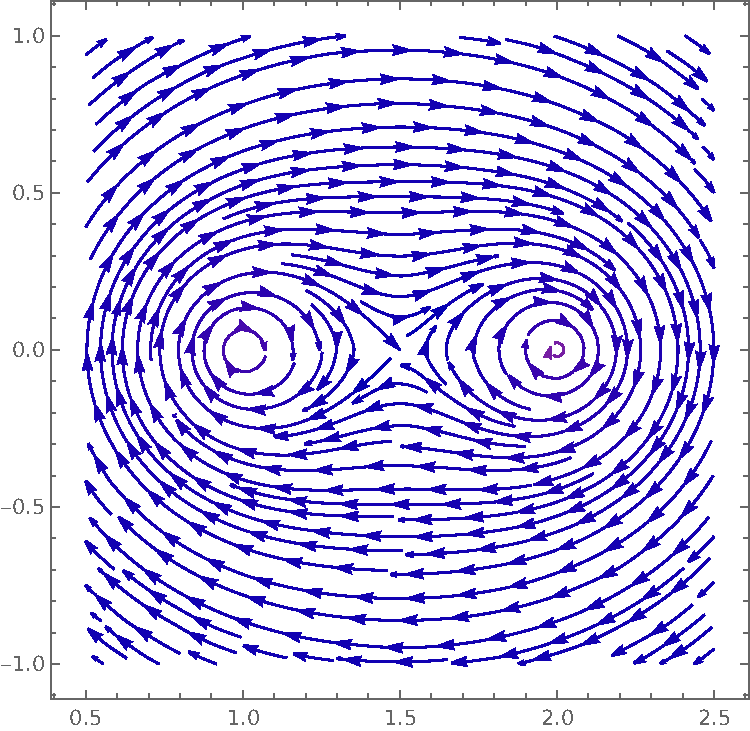
\includegraphics[width=0.7\textwidth]{../Plots/n2_hvf_noInflowNoOutflow_asymmetric.pdf}
  \caption{A plot of $u$ for $M=1$ }
  \label{pl:n2_hvf_noInflowNoOutflow}
\end{figure}

\subsection{An example of inflow on one side and outflow on the other}
Consider the degenerate harmonic function
\begin{align*}
  f_1\colon\C\cong\R^2&\to\R \\
  x&\mapsto \Re\brk*{\brk*{x_1+\iu x_2}^3}\,.
\end{align*}
Since we are only interested in non-degenerate functions we modify this to
\begin{align*}
  f_2(x)= \Re\brk*{\brk*{x_1+\iu x_2}^3}-3\brk*{x_1+x_2}
\end{align*}
Now we set
\begin{align}
  u\colon\R^2\setminus\brk*{\brk[c]*{\vect{-1\\1},\vect{1\\-1}}}&\to\R^2 \\
  x&\mapsto\nabla^\perp f(x)=3\vect{-x_2^2+1\\-x_1^2+1}\label{eq:n2:hvf:InflowOutflow:asymmetric}
\end{align}
As before $u$ is a harmonic vector field. One can show that $u$ has critical points at $\vect{1&1}$ and
$\vect{-1&-1}$. One can further see from figure \ref{pl:n2:hvf:InflowOutflow:asymmetric}
that on a fitting domain with two holes $u$ has inflow from one side and outflow on the other.

\begin{figure}
  \centering
  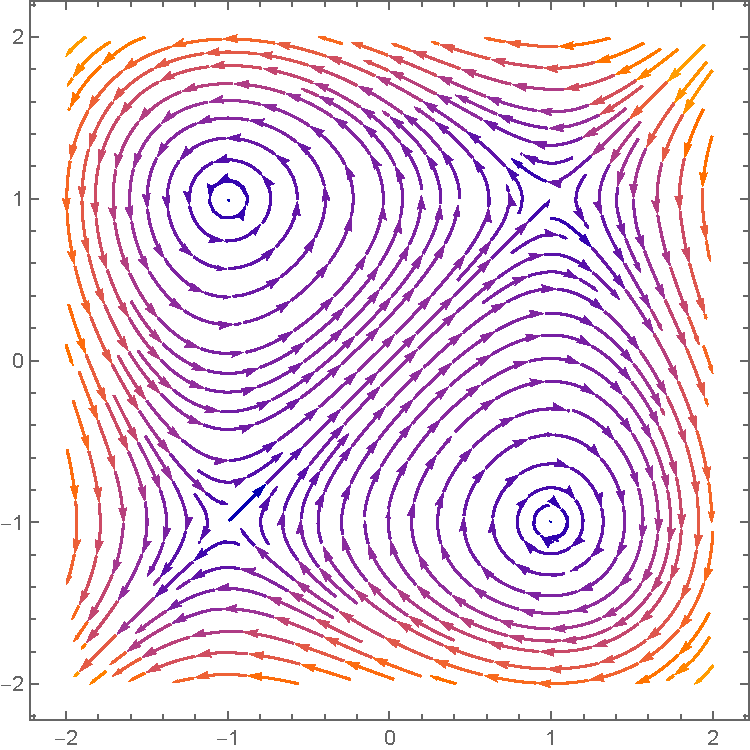
\includegraphics[width=0.7\textwidth]{../Plots/n2_hvf_InflowOutflow_asymmetric.pdf}
  \caption{A plot of $u$ as given by equation \eqref{eq:n2:hvf:InflowOutflow:asymmetric}.}
  \label{pl:n2:hvf:InflowOutflow:asymmetric}
\end{figure}

\ruggedtodo[inline]{Restrict the plots and functions above to suitable domains.}

\newpage

\section{Harmonic functions, $d=3$}

\subsection{The cylinder}

\begin{proposition}
  Let $\Omega=(0,1)\times B_1\subseteq\R^3$ be the cylinder. Let further $f\colon\overline{\Omega}\to\R$ be regular 
  harmonic with no inflow or outflow on the sides 
  $\partial (0,1)\times B_1$, no outflow on $\brk[c]{0}\times B_1$ and no inflow on $\brk[c]{1}\times B_1$. 
  Then $f$ cannot have a critical point.
\end{proposition}
\begin{proof}
  Assume not. Since
  \begin{align*}
    \Delta(\partial_1f)=\partial_1(\Delta f)=0
  \end{align*}
  we have by the maximum principle that $\partial_1 f$ attains its minimum on the boundary $\Sigma$. Since $\partial_1 f(x)=0$ for some interiour point 
  by assumption and $\partial_1 f>0$ on the lids $\brk[c]{x_1=0}\cup\brk[c]{x_1=1}$ there exists a point
  $x\in(0,1)\times S^1$ such that $\partial_1f(x)$ is minimal on $\overline{\Omega}$. But then we have by Hopf's lemma
  that
  \begin{align*}
    0<\nabla (\partial_1f)\cdot n=\partial_1(\nabla f\cdot n)=0\,,
  \end{align*}
  a contradiction.
\end{proof}

\newpage

\subsection{Harmonic vector fields, $d=3$}

\ruggedtodo[inline]{I think the following proof (and statement) is flawed. It needs fixing.}
Mimicking the proof in 2 dimensions we obtain the following proposition.
\begin{proposition}
  Let $\Omega$ have Betti numbers $R_0$,$R_1$ and $R_2$
  Let $u\colon\overline{\Omega}\to\R$ be a regular harmonic vector field without inflow or outflow. Then we have the following relation for
  critical points of $u$
  \begin{align*}
    M_2=M_1
  \end{align*}
\end{proposition}
\begin{proof}[Attempt at proof.]
  As in the two-dimensional case we begin by cutting up the boundary such that $\Omega$ is homeomorphic to the ball with bubbles.
  Once again by a lemma \ruggedtodo[]{now I'm not quite sure about this statement in 3D.} $u$ is the gradient of a harmonic function $u$ on this new domain.
  $f$ has no critical points on the boundary $\Sigma$ and on the cut boundary it fulfils the conditions
  \begin{align}
    \mu_0=\nu_2\qquad \mu_1=\nu_1 \qquad \mu_2=\nu_0 \label{eq:n3:hvf:relationsMuNu}
  \end{align}
  by the same reasoning. We now have the Morse inequalities for $f$ and $-f$
  \begin{align}
    M_2+\mu_2-R_2-M_1-\mu_1+R_1+\mu_0-R_0=0 \label{eq:n3:hvf:MorseInequalities:1} \\
    M_1+\nu_2-R_2-M_2-\nu_1+R_1+\nu_0-R_0=0 \label{eq:n3:hvf:MorseInequalities:2}
  \end{align}
  It then follows by subtracting equation \eqref{eq:n3:hvf:MorseInequalities:2} from \eqref{eq:n3:hvf:MorseInequalities:1}
  and using relations \eqref{eq:n3:hvf:relationsMuNu} that
  \begin{align*}
    2\brk*{M_2-M_1}=0\,.
  \end{align*}
\end{proof}

\newpage

\subsection{Harmonic functions, $d=4$} 
Define the harmonic function 
\begin{align*}
  f\colon B_1\subseteq\R^4&\to \R \\
  x &\mapsto x_1^2+x_2^2-x_3^2-x_4^2\,.
\end{align*}
This has a stagnation point at the origin. We now claim that the sets $\Sigma^+$ and $\Sigma^-$ are both simply connected, i.e.\
we have a tube in $\R^4$ with throughflow and a stagnation point.

\begin{proof}
To prove this claim we observe that the boundary $\partial B_1$ can be parametrised by the coordinates $\bx = (x_2,x_3,x_4)$
for which we have $\abs{\bx}\leq 1$. By the condition
\begin{align}
  \sum_i x_i^2 = 1\label{eq:n4:ball}
\end{align}
on the boundary $\partial B_1$ we have that $x_1$ is then uniquely determined up to sign. Thus we have have defined parametrisations
\begin{align}
  \begin{aligned}\phi_\pm\colon B_1\subseteq\R^3&\to\R \\
  \bx&\mapsto x\text{ such that } \pm x_1\geq0
  \end{aligned}\label{eq:n4:parametrisation}
\end{align}
with inverses $\psi_\pm = \brk*{\phi_\pm}^{-1}$.
We now calculate the gradient of $f$
\begin{align*}
  \nabla f = 2\vect{x_1 & x_2 & -x_3 & -x_4}^\top
\end{align*}
and the normal to $\partial B_1$
\begin{align*}
  n = \vect{x_1 & \cdots & x_4}^\top\,.
\end{align*}
Thus we have $x\in\Sigma^\pm$ iff
\begin{align*}
  0<\pm \nabla f\cdot n = \pm 2\brk*{x_1^2+x_2^2-x_3^2-x_4^2}
\end{align*}
Using condition \eqref{eq:n4:ball} we obtain the equivalent condition
\begin{align*}
  0<\pm 1-2\brk*{x_3^2+x_4^2}
\end{align*}
Define the cylinder
\begin{align*}
  C = \brk[c]*{\bx\in \R^3\colon x_3^2+x_4^2<1/2} = \R\times B_{1/\sqrt{2}}
\end{align*}
If we return to our parametrisation \eqref{eq:n4:parametrisation} we see that we have $\bx\in B_1\cap C$ iff
$\phi_\pm(x)\in \Sigma^+$ and hence 
\begin{align*}
  B_1\cap C=\psi_\pm\brk*{\Sigma^+}\,.
\end{align*}
Analogously  we have 
\begin{align*}
  B_1\setminus C=\psi_\pm\brk*{\Sigma^-}\,.
\end{align*}
The claim then follows from the fact that $\phi$ is a homeomorphism onto its image and $x_1=0$ is 
equivalent to $\bx\in \partial B_1\subseteq \R^2$. The situation is depicted in figure \ref{fi:n4_sigma}.

\begin{figure}[h]
  \centering
  \def\svgwidth{0.7\textwidth}
  \input{../Figures/n4_sigma.pdf_tex}
  \caption{Visualisation of the situation.}
  \label{fi:n4_sigma}
\end{figure}
\end{proof}

\clearpage

% TODO: potentially add Irwin, smooth dynamical systems
\section{Bibliography}
\nocite{*}
%Main source
%\printbibliography[heading=none, keyword={main}]
%\noindent Other sources
\printbibliography[heading=none]


\end{document}